\label{Chapter4}

\chapter{Experimental Validation}

\section{Scope of Experiments}

The purpose of the experiments is to validate the proposed system as
well as its robustness in various terrains and configurations.
Since the autonomous navigation of the robot is out of the scope of this
thesis, the mapping procedure is only indirectly validated as part of the
SLAM system.
Thus, the main focus of the experiments is the relative and absolute
localization techniques that were developed.

\subsection{Data Collection}

The performed experiments were executed by means of
\textit{Software In the Loop} (SIL) tests using precollected data.
The data were collected by the Planetary Robotics Lab team of the European
Space Agency as part of a two week test campaign that took
place in the Minas de San Jose desert in Tenerife, Spain with the aim to
validate the integration of the HDPR rover (Section \ref{hdpr_rover}) and
provide data for future research projects.

For that reason, the collected dataset contains samples from:
\begin{enumerate*}[label=(\roman*)]
        \item three stereo camera sensors
        \item IMU sensor
        \item point clouds reconstructed from drone imagery
        \item GPS sensor.
\end{enumerate*}
These samples are used both as input to our system and as ground truth
information.

The environment in which the test data were collected, was chosen with
the aim to bear close resemblance to rough planetary terrains,
specifically to the one of Mars.
In particular, various geological properties such as the distribution
and the shape of the rocks is similar to the Martian terrain.

Finally, the speed of the robot in these datasets was chosen to be close
to the $\SI{10}{\cm}$ value, considering the long-range traverses it was
required to cover.
As such, for the first two experiments, the size of the local map is fixed at
$\SI{20 x 20}{\m}$ and its resolution at $\SI{10}{\cm \per cell}$,
while for the global map we presumed the resolution to be fixed at
$\SI{50}{\cm \per cell}$.
In the third experiment, the performance of our approach is validated against
these parameters, hence they are variable.

% TODO: add figures showing the said environment/traverses from maps/drone

\subsection{Metrics} \label{metrics}

To quantify the experimental results and evaluate the outputs of the system,
it is necessary to introduce certain metrics:
\begin{itemize}
    \item \textbf{Mean square error (MSE) of pose graph}:
        This is a straightforward metric for benchmarking SLAM algorithms
        and can be defined as
        \begin{equation}
            \varepsilon_{MSE} (\hat{x}_{1:T}) = \frac{1}{T}
            \sum\limits_{t=1}^T (\hat{x}_t \ominus x_t)^2
        \end{equation}
        where
        $\hat{x}_{1:T}$ is the estimated pose graph,
        $x_{1:T}$ is the ground truth pose graph,
        $T$ is the number of samples and
        $x_i \ominus x_j$ is the distance between two poses.

        % TODO(ref): "On Measuring the Accuracy of SLAM Algorithms" paper

    \item \textbf{Root mean square deviation (RMSD) of pose graph}:
        Similarly to the MSE metric, this metric expresses the sample
        standard deviation of the differences between the estimated and the
        ground truth poses and can be defined as
        \begin{equation}
            \varepsilon_{RMSD} (\hat{x}_{1:T}) = \sqrt{\frac{1}{T}
            \sum\limits_{t=1}^T (y_t - \varepsilon_{MSE})^2}
        \end{equation}
        where $y_t$ is defined as $\hat{x}_t \ominus x_t$.

    % \item \textbf{Execution time of scan matching}:
    % \item \textbf{Execution time of map matching}:
\end{itemize}

\section{Experiments on Pose Estimation}

\subsection{Relative Localization Results}

The purpose of this experiment is to test the accuracy of the Pose Estimation
module (see Section \ref{pose_estimation}) and evaluate its capabilities
in relative localization (short-range) scenarios.
To accomplish that, we will carry out each experiment in separate
environments and use different parameter sets with the aim of examining the
system's sensitivity as well as finding an optimal parameter configuration.

The main parameters that we will tune during the experiments are all related
to the particle filter and include
\begin{enumerate*}[label=(\roman*)]
        \item the number of particles used
        \item the resampling frequency
        \item the standard deviation of the Gaussian noise
            added to each particle.
\end{enumerate*}
With regard to the environment, since the existence of features affects the
outcome of the scan matching which is performed to update the weight
of each particle (see Section \ref{pf_update}), it is necessary to
repeat the tests in terrains with distinct rock distributions.
Finally, the expected error of the estimated pose should
ideally be less than the size of one cell of the local map, so as to
ensure that the robot can distinguish the environment's obstacles with
a high-level of certainty.

\subsubsection{Scenario 1}

Figure \ref{fig:terrain_1} present a view of the evaluated terrain of the first
scenario.
The terrain is depicted in the form of one dense point cloud which was
reconstructed from drone imagery.
% TODO: add 3D (not bird's eye view) of terrain from drone map PLY
The bird's eye view in Figure \ref{fig:bird_1} shows the traverse of the
robot in this scenario and compares the ground truth path, the one
from raw visual odometry and the one from the pose estimation.
% TODO: add bird's eye view with: ground truth/Odometry/PF estimate
% TODO: quickly discuss result

\begin{figure}
    \centering
    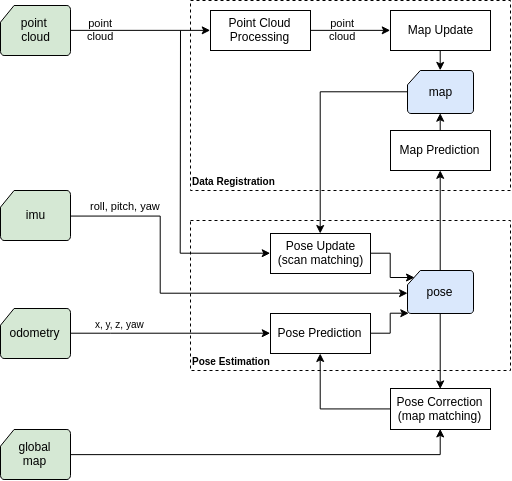
\includegraphics[scale=0.4,draft]{high_level_design_diagram}
    % \includegraphics[scale=0.4]{scenario_1_terrain}
    \caption[Name]{
        Description
    }
    \label{fig:terrain_1}
\end{figure}

\begin{figure}
    \centering
    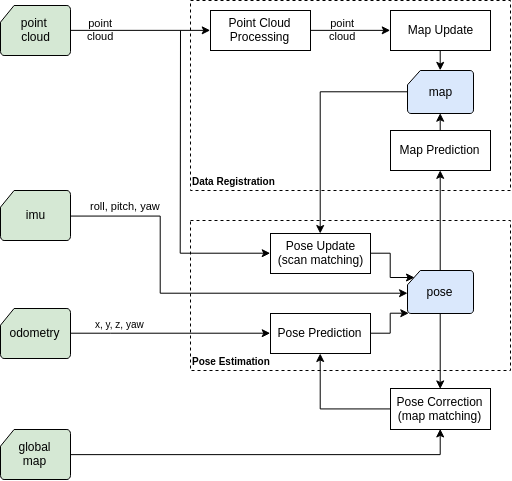
\includegraphics[scale=0.4,draft]{high_level_design_diagram}
    % \includegraphics[scale=0.4]{scenario_1_bird}
    \caption[Name]{
        Description
    }
    \label{fig:bird_1}
\end{figure}

In particular, the effect of the number of particles used has on
the outcome is shown in the comparison plots in Figures
\ref{fig:mean_error_vs_particles_1} and \ref{fig:std_error_vs_particles_1}.
% TODO: add plot showing the mean error vs particles
% TODO: add plot showing the std error vs particles
% TODO: quickly discuss result

\begin{figure}
    \centering
    % This file was created by matplotlib2tikz v0.6.15.
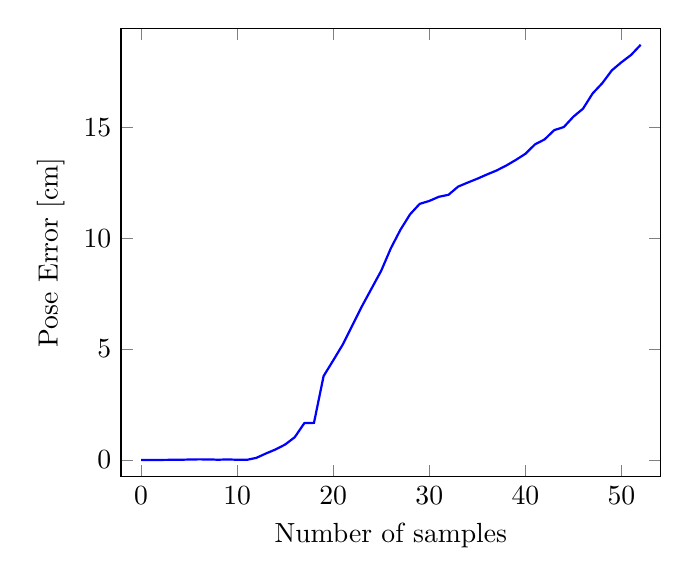
\begin{tikzpicture}

\begin{axis}[
xlabel={Number of samples},
ylabel={Pose Error [cm]},
xmin=-2.08, xmax=54.08,
ymin=-0.748415252462355, ymax=19.4588330238832,
axis on top,
tick pos=both
]
\addplot [thick, blue, forget plot]
table {%
0 1.35036525754666e-06
1 0.000125138484529261
2 0.00102913069024886
3 0.00479680696188859
4 0.00916186830903526
5 0.0174038646274569
6 0.0262520837326282
7 0.0221047623524557
8 0.0111512199617931
9 0.0201210813050887
10 0.0103041075482047
11 0.00407634710390544
12 0.0926150953094736
13 0.290839276112037
14 0.472058763443635
15 0.694965291952438
16 1.02500944562528
17 1.66024002284578
18 1.6709268730271
19 3.77884873435007
20 4.48456421300077
21 5.20350845261926
22 6.06989521034351
23 6.93276612800943
24 7.7323716638851
25 8.52934043849111
26 9.54013041030872
27 10.3761549548947
28 11.070579373762
29 11.5411081034943
30 11.6740911712709
31 11.8615182982339
32 11.9506618950995
33 12.319284997278
34 12.5018994038963
35 12.6755111193714
36 12.8659334573785
37 13.0459756265849
38 13.2666821205177
39 13.5203293101627
40 13.796881010613
41 14.2231742569443
42 14.4465486146409
43 14.8645806490604
44 15.0041899388582
45 15.4721867591002
46 15.8327233804673
47 16.518800150712
48 16.9798252351286
49 17.5599615612027
50 17.9252447964595
51 18.2535561358361
52 18.7104164210556
};
\end{axis}

\end{tikzpicture}

    % \input{Plots/mean_error_vs_particles_1.tex}
    \caption[Name]{
        Description
    }
    \label{fig:mean_error_vs_particles_1}
\end{figure}

\begin{figure}
    \centering
    % This file was created by matplotlib2tikz v0.6.15.
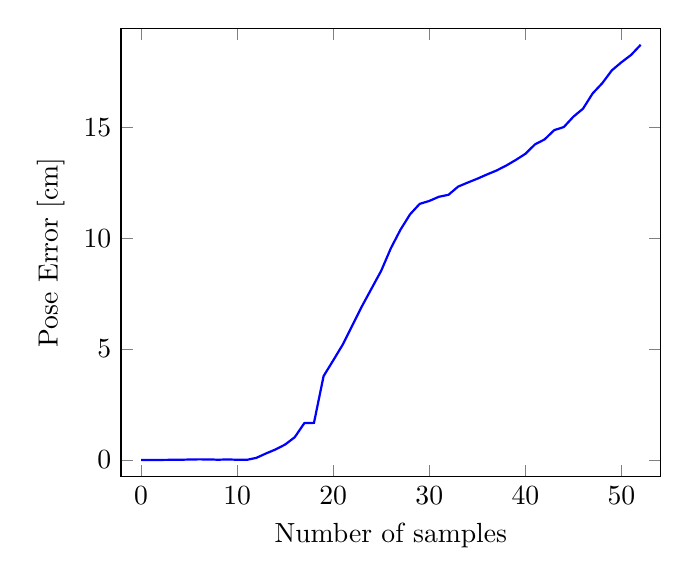
\begin{tikzpicture}

\begin{axis}[
xlabel={Number of samples},
ylabel={Pose Error [cm]},
xmin=-2.08, xmax=54.08,
ymin=-0.748415252462355, ymax=19.4588330238832,
axis on top,
tick pos=both
]
\addplot [thick, blue, forget plot]
table {%
0 1.35036525754666e-06
1 0.000125138484529261
2 0.00102913069024886
3 0.00479680696188859
4 0.00916186830903526
5 0.0174038646274569
6 0.0262520837326282
7 0.0221047623524557
8 0.0111512199617931
9 0.0201210813050887
10 0.0103041075482047
11 0.00407634710390544
12 0.0926150953094736
13 0.290839276112037
14 0.472058763443635
15 0.694965291952438
16 1.02500944562528
17 1.66024002284578
18 1.6709268730271
19 3.77884873435007
20 4.48456421300077
21 5.20350845261926
22 6.06989521034351
23 6.93276612800943
24 7.7323716638851
25 8.52934043849111
26 9.54013041030872
27 10.3761549548947
28 11.070579373762
29 11.5411081034943
30 11.6740911712709
31 11.8615182982339
32 11.9506618950995
33 12.319284997278
34 12.5018994038963
35 12.6755111193714
36 12.8659334573785
37 13.0459756265849
38 13.2666821205177
39 13.5203293101627
40 13.796881010613
41 14.2231742569443
42 14.4465486146409
43 14.8645806490604
44 15.0041899388582
45 15.4721867591002
46 15.8327233804673
47 16.518800150712
48 16.9798252351286
49 17.5599615612027
50 17.9252447964595
51 18.2535561358361
52 18.7104164210556
};
\end{axis}

\end{tikzpicture}

    % \input{Plots/std_error_vs_particles_1.tex}
    \caption[Name]{
        Description
    }
    \label{fig:std_error_vs_particles_1}
\end{figure}

Furthermore, the plots in Figures \ref{fig:mean_error_vs_resampling_1} and
\ref{fig:std_error_vs_resampling_1} represent the same errors as the previous
plots, with the difference that the number of particles is fixed to the
value of 50 and the resampling frequency is the variable parameter.
% TODO: add plot showing the mean error vs resampling
% TODO: add plot showing the std error vs resampling
% TODO: quickly discuss result

\begin{figure}
    \centering
    % This file was created by matplotlib2tikz v0.6.15.
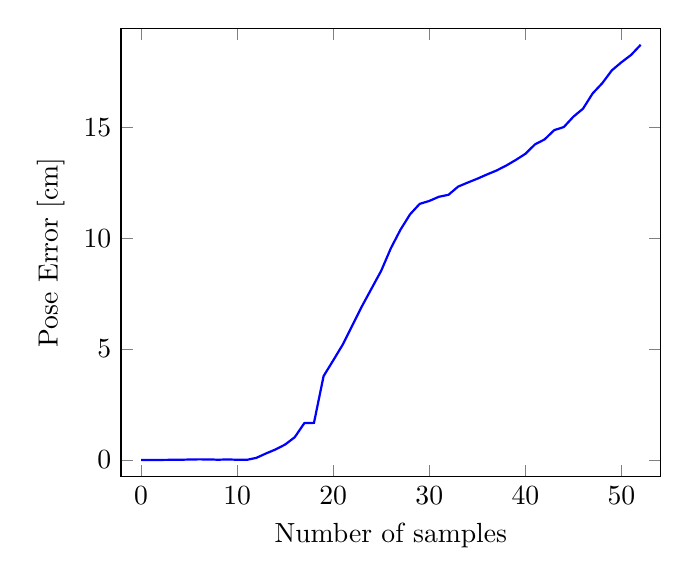
\begin{tikzpicture}

\begin{axis}[
xlabel={Number of samples},
ylabel={Pose Error [cm]},
xmin=-2.08, xmax=54.08,
ymin=-0.748415252462355, ymax=19.4588330238832,
axis on top,
tick pos=both
]
\addplot [thick, blue, forget plot]
table {%
0 1.35036525754666e-06
1 0.000125138484529261
2 0.00102913069024886
3 0.00479680696188859
4 0.00916186830903526
5 0.0174038646274569
6 0.0262520837326282
7 0.0221047623524557
8 0.0111512199617931
9 0.0201210813050887
10 0.0103041075482047
11 0.00407634710390544
12 0.0926150953094736
13 0.290839276112037
14 0.472058763443635
15 0.694965291952438
16 1.02500944562528
17 1.66024002284578
18 1.6709268730271
19 3.77884873435007
20 4.48456421300077
21 5.20350845261926
22 6.06989521034351
23 6.93276612800943
24 7.7323716638851
25 8.52934043849111
26 9.54013041030872
27 10.3761549548947
28 11.070579373762
29 11.5411081034943
30 11.6740911712709
31 11.8615182982339
32 11.9506618950995
33 12.319284997278
34 12.5018994038963
35 12.6755111193714
36 12.8659334573785
37 13.0459756265849
38 13.2666821205177
39 13.5203293101627
40 13.796881010613
41 14.2231742569443
42 14.4465486146409
43 14.8645806490604
44 15.0041899388582
45 15.4721867591002
46 15.8327233804673
47 16.518800150712
48 16.9798252351286
49 17.5599615612027
50 17.9252447964595
51 18.2535561358361
52 18.7104164210556
};
\end{axis}

\end{tikzpicture}

    % \input{Plots/mean_error_vs_resampling_1.tex}
    \caption[Name]{
        Description
    }
    \label{fig:mean_error_vs_resampling_1}
\end{figure}

\begin{figure}
    \centering
    % This file was created by matplotlib2tikz v0.6.15.
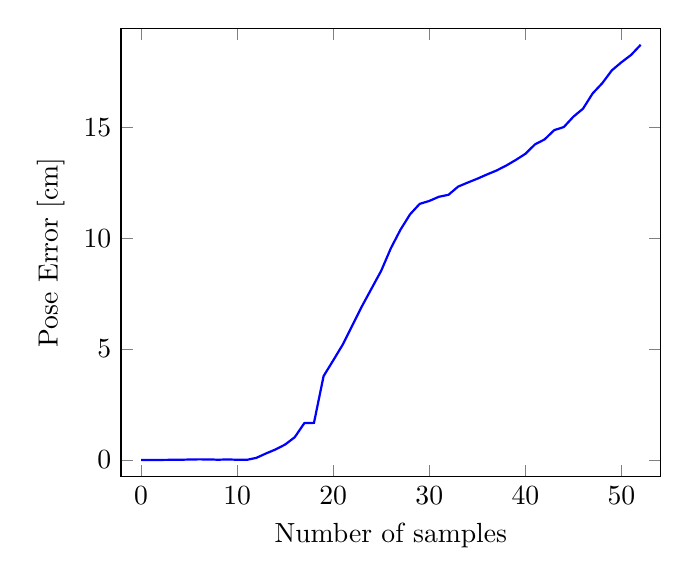
\begin{tikzpicture}

\begin{axis}[
xlabel={Number of samples},
ylabel={Pose Error [cm]},
xmin=-2.08, xmax=54.08,
ymin=-0.748415252462355, ymax=19.4588330238832,
axis on top,
tick pos=both
]
\addplot [thick, blue, forget plot]
table {%
0 1.35036525754666e-06
1 0.000125138484529261
2 0.00102913069024886
3 0.00479680696188859
4 0.00916186830903526
5 0.0174038646274569
6 0.0262520837326282
7 0.0221047623524557
8 0.0111512199617931
9 0.0201210813050887
10 0.0103041075482047
11 0.00407634710390544
12 0.0926150953094736
13 0.290839276112037
14 0.472058763443635
15 0.694965291952438
16 1.02500944562528
17 1.66024002284578
18 1.6709268730271
19 3.77884873435007
20 4.48456421300077
21 5.20350845261926
22 6.06989521034351
23 6.93276612800943
24 7.7323716638851
25 8.52934043849111
26 9.54013041030872
27 10.3761549548947
28 11.070579373762
29 11.5411081034943
30 11.6740911712709
31 11.8615182982339
32 11.9506618950995
33 12.319284997278
34 12.5018994038963
35 12.6755111193714
36 12.8659334573785
37 13.0459756265849
38 13.2666821205177
39 13.5203293101627
40 13.796881010613
41 14.2231742569443
42 14.4465486146409
43 14.8645806490604
44 15.0041899388582
45 15.4721867591002
46 15.8327233804673
47 16.518800150712
48 16.9798252351286
49 17.5599615612027
50 17.9252447964595
51 18.2535561358361
52 18.7104164210556
};
\end{axis}

\end{tikzpicture}

    % \input{Plots/std_error_vs_resampling_1.tex}
    \caption[Name]{
        Description
    }
    \label{fig:std_error_vs_resampling_1}
\end{figure}

For the purpose of further quantifying the results of this scenario altogether,
we calculate the $MSE$ and $RMSD$ metrics (defined in Section \ref{metrics})
for the parameter sets that were used to generate the above plots.
The values of these metrics are presented in Table \ref{table:metrics_1}.
% TODO: add table with MSE/RMSD vs {1particle+5resampling, 50p+5r, 100p+5r, ..}
% TODO: quickly discuss result

\begin{table}
    \centering
    \begin{tabular}{| c | c || c | c |}
        \hline
        Particle Number & Resampling frequency & MSE & RMSD \\
        \hline
        \hline
        50 & 1 & 100 & 10 \\
        50 & 5 & 100 & 10 \\
        50 & 20 & 100 & 10 \\
        100 & 1 & 100 & 10 \\
        100 & 1 & 100 & 10 \\
        100 & 5 & 100 & 10 \\
        200 & 20 & 100 & 10 \\
        200 & 5 & 100 & 10 \\
        200 & 20 & 100 & 10 \\
        \hline
    \end{tabular}
    \caption[Name]{
        Description
    }
    \label{table:metrics_1}
\end{table}

% TODO: discuss the above results and what are the advantages/drawbacks while tuning each parameter

\subsubsection{Scenario 2}

In the second scenario, a more sparse terrain was evaluated with a focus on
quantifying the robustness of the developed scan matching technique, which
is directly affected by the existence of features.
Figure \ref{fig:terrain_2} presents the aforementioned terrain and
Figure \ref{fig:bird_2} shows the robot's traverse in it.
% TODO: add bird's eye view with: ground truth/Odometry/PF estimate
% TODO: quickly discuss result

\begin{figure}
    \centering
    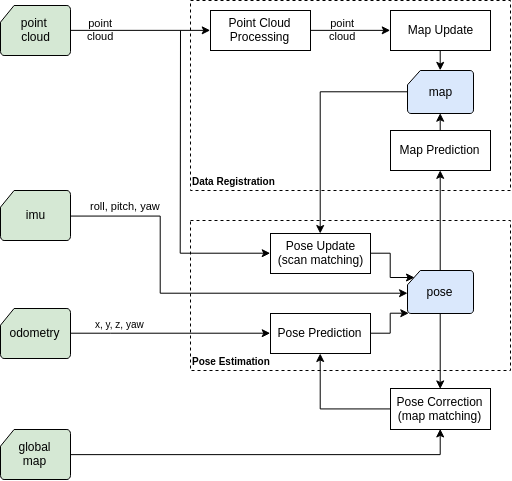
\includegraphics[scale=0.4,draft]{high_level_design_diagram}
    % \includegraphics[scale=0.4]{scenario_2_terrain}
    \caption[Name]{
        Description
    }
    \label{fig:terrain_2}
\end{figure}

\begin{figure}
    \centering
    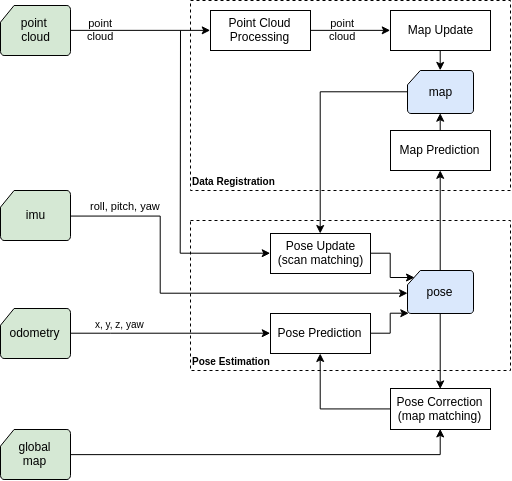
\includegraphics[scale=0.4,draft]{high_level_design_diagram}
    % \includegraphics[scale=0.4]{scenario_2_bird}
    \caption[Name]{
        Description
    }
    \label{fig:bird_2}
\end{figure}

In the same manner as in the first scenario, we carry out this experiment
against various parameter configurations.
By tuning the number of particles, we received the results shown in Figures
\ref{fig:mean_error_vs_particles_2} and \ref{fig:std_error_vs_particles_2}.
Accordingly, tuning the resampling frequency results to the plots shown in
Figures \ref{fig:mean_error_vs_resampling_2} and
\ref{fig:std_error_vs_resampling_2}.
% TODO: add plot showing the mean error vs particles
% TODO: add plot showing the std error vs particles
% TODO: add plot showing the mean error vs resampling
% TODO: add plot showing the std error vs resampling
% TODO: quickly discuss result

\begin{figure}
    \centering
    % This file was created by matplotlib2tikz v0.6.15.
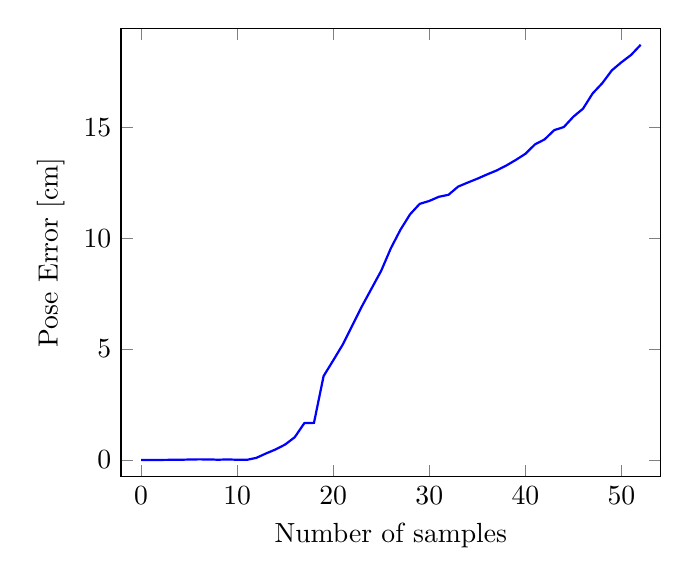
\begin{tikzpicture}

\begin{axis}[
xlabel={Number of samples},
ylabel={Pose Error [cm]},
xmin=-2.08, xmax=54.08,
ymin=-0.748415252462355, ymax=19.4588330238832,
axis on top,
tick pos=both
]
\addplot [thick, blue, forget plot]
table {%
0 1.35036525754666e-06
1 0.000125138484529261
2 0.00102913069024886
3 0.00479680696188859
4 0.00916186830903526
5 0.0174038646274569
6 0.0262520837326282
7 0.0221047623524557
8 0.0111512199617931
9 0.0201210813050887
10 0.0103041075482047
11 0.00407634710390544
12 0.0926150953094736
13 0.290839276112037
14 0.472058763443635
15 0.694965291952438
16 1.02500944562528
17 1.66024002284578
18 1.6709268730271
19 3.77884873435007
20 4.48456421300077
21 5.20350845261926
22 6.06989521034351
23 6.93276612800943
24 7.7323716638851
25 8.52934043849111
26 9.54013041030872
27 10.3761549548947
28 11.070579373762
29 11.5411081034943
30 11.6740911712709
31 11.8615182982339
32 11.9506618950995
33 12.319284997278
34 12.5018994038963
35 12.6755111193714
36 12.8659334573785
37 13.0459756265849
38 13.2666821205177
39 13.5203293101627
40 13.796881010613
41 14.2231742569443
42 14.4465486146409
43 14.8645806490604
44 15.0041899388582
45 15.4721867591002
46 15.8327233804673
47 16.518800150712
48 16.9798252351286
49 17.5599615612027
50 17.9252447964595
51 18.2535561358361
52 18.7104164210556
};
\end{axis}

\end{tikzpicture}

    % \input{Plots/mean_error_vs_particles_2.tex}
    \caption[Name]{
        Description
    }
    \label{fig:mean_error_vs_particles_2}
\end{figure}

\begin{figure}
    \centering
    % This file was created by matplotlib2tikz v0.6.15.
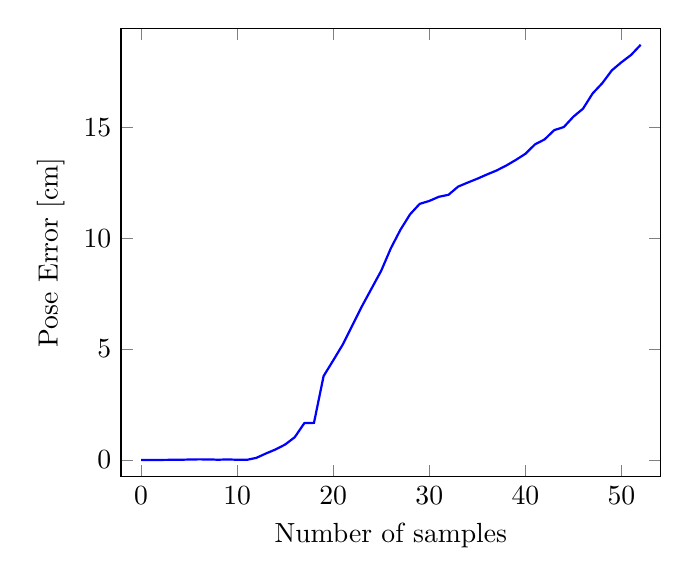
\begin{tikzpicture}

\begin{axis}[
xlabel={Number of samples},
ylabel={Pose Error [cm]},
xmin=-2.08, xmax=54.08,
ymin=-0.748415252462355, ymax=19.4588330238832,
axis on top,
tick pos=both
]
\addplot [thick, blue, forget plot]
table {%
0 1.35036525754666e-06
1 0.000125138484529261
2 0.00102913069024886
3 0.00479680696188859
4 0.00916186830903526
5 0.0174038646274569
6 0.0262520837326282
7 0.0221047623524557
8 0.0111512199617931
9 0.0201210813050887
10 0.0103041075482047
11 0.00407634710390544
12 0.0926150953094736
13 0.290839276112037
14 0.472058763443635
15 0.694965291952438
16 1.02500944562528
17 1.66024002284578
18 1.6709268730271
19 3.77884873435007
20 4.48456421300077
21 5.20350845261926
22 6.06989521034351
23 6.93276612800943
24 7.7323716638851
25 8.52934043849111
26 9.54013041030872
27 10.3761549548947
28 11.070579373762
29 11.5411081034943
30 11.6740911712709
31 11.8615182982339
32 11.9506618950995
33 12.319284997278
34 12.5018994038963
35 12.6755111193714
36 12.8659334573785
37 13.0459756265849
38 13.2666821205177
39 13.5203293101627
40 13.796881010613
41 14.2231742569443
42 14.4465486146409
43 14.8645806490604
44 15.0041899388582
45 15.4721867591002
46 15.8327233804673
47 16.518800150712
48 16.9798252351286
49 17.5599615612027
50 17.9252447964595
51 18.2535561358361
52 18.7104164210556
};
\end{axis}

\end{tikzpicture}

    % \input{Plots/std_error_vs_particles_2.tex}
    \caption[Name]{
        Description
    }
    \label{fig:std_error_vs_particles_2}
\end{figure}

\begin{figure}
    \centering
    % This file was created by matplotlib2tikz v0.6.15.
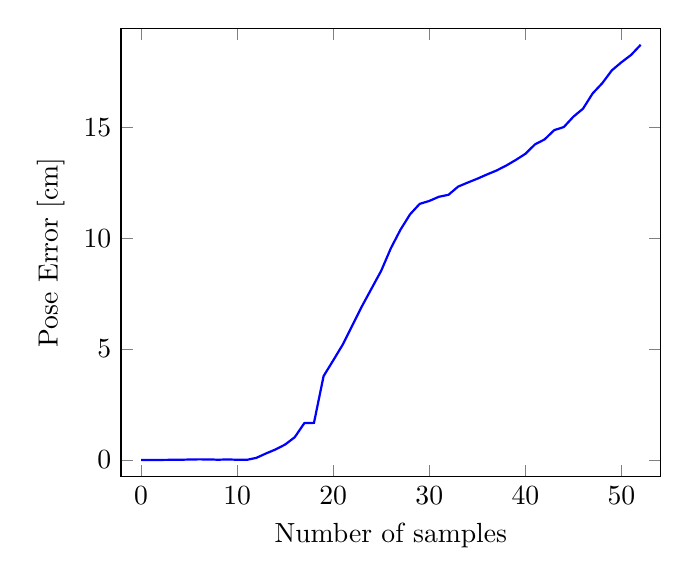
\begin{tikzpicture}

\begin{axis}[
xlabel={Number of samples},
ylabel={Pose Error [cm]},
xmin=-2.08, xmax=54.08,
ymin=-0.748415252462355, ymax=19.4588330238832,
axis on top,
tick pos=both
]
\addplot [thick, blue, forget plot]
table {%
0 1.35036525754666e-06
1 0.000125138484529261
2 0.00102913069024886
3 0.00479680696188859
4 0.00916186830903526
5 0.0174038646274569
6 0.0262520837326282
7 0.0221047623524557
8 0.0111512199617931
9 0.0201210813050887
10 0.0103041075482047
11 0.00407634710390544
12 0.0926150953094736
13 0.290839276112037
14 0.472058763443635
15 0.694965291952438
16 1.02500944562528
17 1.66024002284578
18 1.6709268730271
19 3.77884873435007
20 4.48456421300077
21 5.20350845261926
22 6.06989521034351
23 6.93276612800943
24 7.7323716638851
25 8.52934043849111
26 9.54013041030872
27 10.3761549548947
28 11.070579373762
29 11.5411081034943
30 11.6740911712709
31 11.8615182982339
32 11.9506618950995
33 12.319284997278
34 12.5018994038963
35 12.6755111193714
36 12.8659334573785
37 13.0459756265849
38 13.2666821205177
39 13.5203293101627
40 13.796881010613
41 14.2231742569443
42 14.4465486146409
43 14.8645806490604
44 15.0041899388582
45 15.4721867591002
46 15.8327233804673
47 16.518800150712
48 16.9798252351286
49 17.5599615612027
50 17.9252447964595
51 18.2535561358361
52 18.7104164210556
};
\end{axis}

\end{tikzpicture}

    % \input{Plots/mean_error_vs_resampling_2.tex}
    \caption[Name]{
        Description
    }
    \label{fig:mean_error_vs_resampling_2}
\end{figure}

\begin{figure}
    \centering
    % This file was created by matplotlib2tikz v0.6.15.
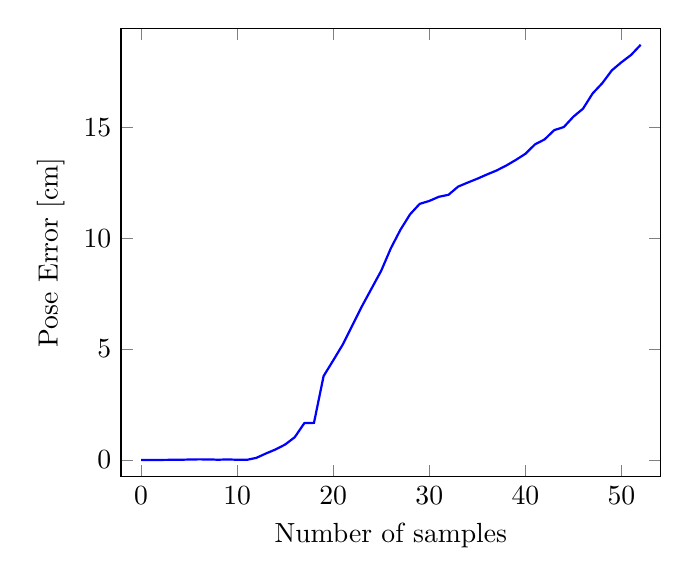
\begin{tikzpicture}

\begin{axis}[
xlabel={Number of samples},
ylabel={Pose Error [cm]},
xmin=-2.08, xmax=54.08,
ymin=-0.748415252462355, ymax=19.4588330238832,
axis on top,
tick pos=both
]
\addplot [thick, blue, forget plot]
table {%
0 1.35036525754666e-06
1 0.000125138484529261
2 0.00102913069024886
3 0.00479680696188859
4 0.00916186830903526
5 0.0174038646274569
6 0.0262520837326282
7 0.0221047623524557
8 0.0111512199617931
9 0.0201210813050887
10 0.0103041075482047
11 0.00407634710390544
12 0.0926150953094736
13 0.290839276112037
14 0.472058763443635
15 0.694965291952438
16 1.02500944562528
17 1.66024002284578
18 1.6709268730271
19 3.77884873435007
20 4.48456421300077
21 5.20350845261926
22 6.06989521034351
23 6.93276612800943
24 7.7323716638851
25 8.52934043849111
26 9.54013041030872
27 10.3761549548947
28 11.070579373762
29 11.5411081034943
30 11.6740911712709
31 11.8615182982339
32 11.9506618950995
33 12.319284997278
34 12.5018994038963
35 12.6755111193714
36 12.8659334573785
37 13.0459756265849
38 13.2666821205177
39 13.5203293101627
40 13.796881010613
41 14.2231742569443
42 14.4465486146409
43 14.8645806490604
44 15.0041899388582
45 15.4721867591002
46 15.8327233804673
47 16.518800150712
48 16.9798252351286
49 17.5599615612027
50 17.9252447964595
51 18.2535561358361
52 18.7104164210556
};
\end{axis}

\end{tikzpicture}

    % \input{Plots/std_error_vs_resampling_2.tex}
    \caption[Name]{
        Description
    }
    \label{fig:std_error_vs_resampling_2}
\end{figure}

Finally, we evaluate the overall performance of the system in this scenario
using the $MSE$ and $RMSD$ metrics as shown in Table \ref{table:metrics_2}.
% TODO: add table with MSE/RMSD vs {1particle+5resampling, 50p+5r, 100p+5r, ..}
% TODO: quickly discuss result

% TODO: discuss the robustness of the scan matching technique of the PF

\section{Experiments on Global Map Matching}

\subsection{Absolute Localization Results}

Contrary to relative localization, which is the ability to track the robot's
pose, absolute localization is the ability to maintain the tracked pose
which diverges due to accumulated errors over time.
For this purpose, we will test the system in long-range
scenarios where localization drifts are manifested and assess the robustness
of the Pose Correction module (see Section \ref{pose_correction})

Similarly to the pose estimation experiments, the expected error of the
corrected pose should ideally be less than the size of one cell of the global
map, in consideration of the fact that the global map's resolution is higher
than the resolution of the local map.

\subsubsection{Scenario 1}

In the first scenario we evaluate the pose correction functionality in
a feature-rich terrain, i.e. a terrain that contains several elevation
features such as rocks.
Figure \ref{fig:terrain_3} presents the view of such terrain as a dense
point cloud and Figure \ref{fig:bird_3} shows the traverse inside it.
In addition, we present the orthographic projections of the global
elevation map (Figure \ref{fig:global_elevation_map_1}) and its gradient
(Figure \ref{fig:global_gradient_map_1}).
% TODO: add 3D (not bird's eye view) of terrain from drone map PLY
% TODO: add bird's eye view with: ground truth/no correction/correction

\begin{figure}
    \centering
    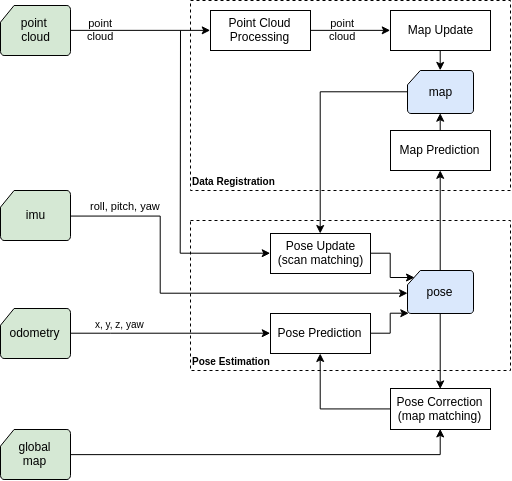
\includegraphics[scale=0.4,draft]{high_level_design_diagram}
    % \includegraphics[scale=0.4]{scenario_3_terrain}
    \caption[Name]{
        Description
    }
    \label{fig:terrain_3}
\end{figure}

\begin{figure}
    \centering
    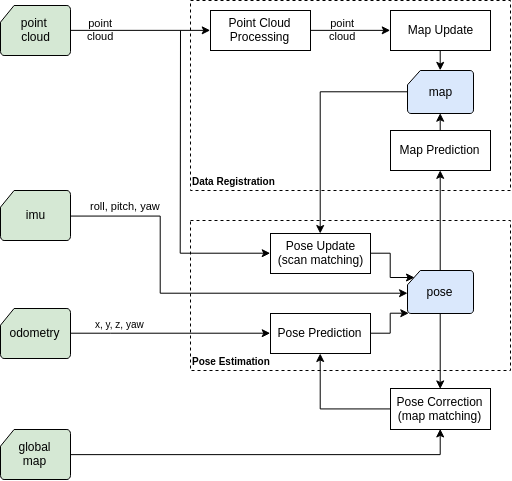
\includegraphics[scale=0.4,draft]{high_level_design_diagram}
    % \includegraphics[scale=0.4]{scenario_3_bird}
    \caption[Name]{
        Description
    }
    \label{fig:bird_3}
\end{figure}

\begin{figure}
    \centering
    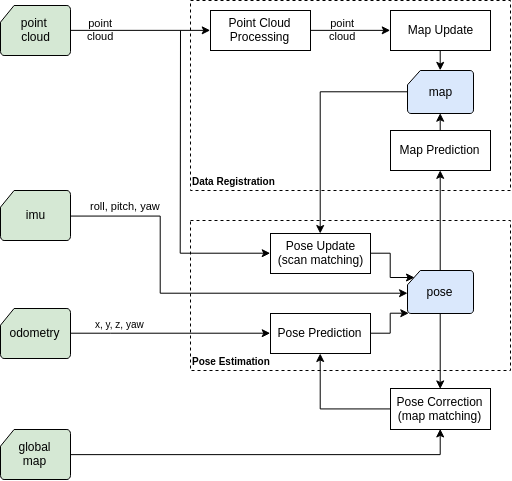
\includegraphics[scale=0.4,draft]{high_level_design_diagram}
    % \includegraphics[scale=0.4]{global_elevation_map_1}
    \caption[Name]{
        Description
    }
    \label{fig:global_elevation_map_1}
\end{figure}

\begin{figure}
    \centering
    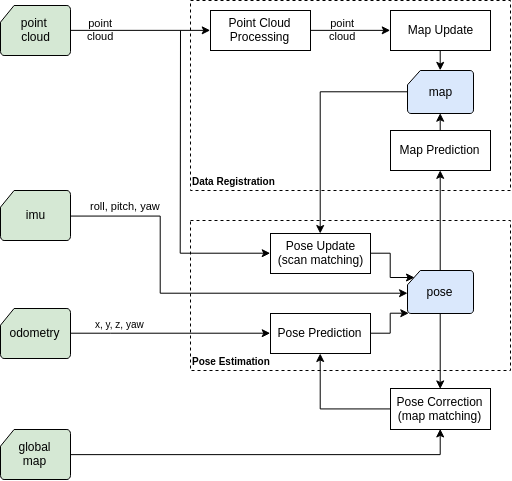
\includegraphics[scale=0.4,draft]{high_level_design_diagram}
    % \includegraphics[scale=0.4]{global_gradient_map_1}
    \caption[Name]{
        Description
    }
    \label{fig:global_gradient_map_1}
\end{figure}

% TODO: add orthographic projection with global elevation map and its gradient

The correction of the accumulated error is more visible in the plot of
Figure \ref{fig:pose_correction_error_1}.
The score of the yielded result from the global to local map matching,
as well as the rate of correction, are visible in Table
\ref{table:pose_correction_1}.
We can notice that the score of the match is $97\%$ (where $100\%$ is a
perfect match - as defined in Section \ref{map_matching}) and since
the matching threshold was set to $95\%$, the match is accepted and used
to correct the robot's pose by $99\%$.
% TODO: add plot showing the pose error over time
% TODO: add table with the matching accuracy and percentage/rate of correction

\begin{figure}
    \centering
    % This file was created by matplotlib2tikz v0.6.15.
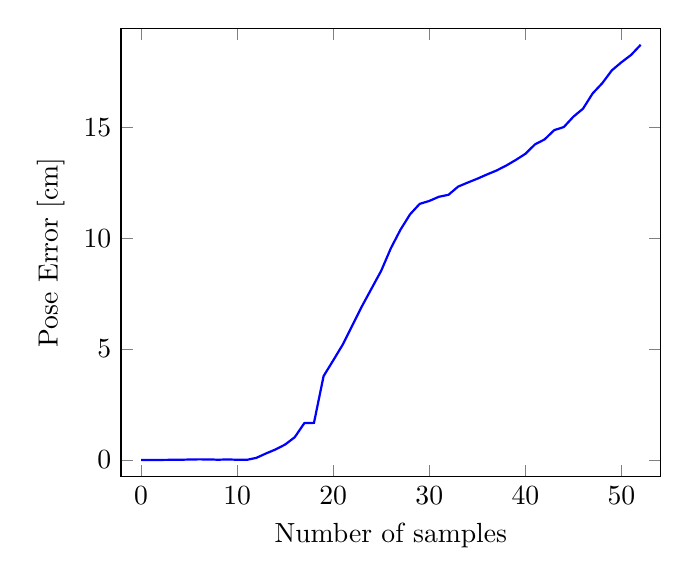
\begin{tikzpicture}

\begin{axis}[
xlabel={Number of samples},
ylabel={Pose Error [cm]},
xmin=-2.08, xmax=54.08,
ymin=-0.748415252462355, ymax=19.4588330238832,
axis on top,
tick pos=both
]
\addplot [thick, blue, forget plot]
table {%
0 1.35036525754666e-06
1 0.000125138484529261
2 0.00102913069024886
3 0.00479680696188859
4 0.00916186830903526
5 0.0174038646274569
6 0.0262520837326282
7 0.0221047623524557
8 0.0111512199617931
9 0.0201210813050887
10 0.0103041075482047
11 0.00407634710390544
12 0.0926150953094736
13 0.290839276112037
14 0.472058763443635
15 0.694965291952438
16 1.02500944562528
17 1.66024002284578
18 1.6709268730271
19 3.77884873435007
20 4.48456421300077
21 5.20350845261926
22 6.06989521034351
23 6.93276612800943
24 7.7323716638851
25 8.52934043849111
26 9.54013041030872
27 10.3761549548947
28 11.070579373762
29 11.5411081034943
30 11.6740911712709
31 11.8615182982339
32 11.9506618950995
33 12.319284997278
34 12.5018994038963
35 12.6755111193714
36 12.8659334573785
37 13.0459756265849
38 13.2666821205177
39 13.5203293101627
40 13.796881010613
41 14.2231742569443
42 14.4465486146409
43 14.8645806490604
44 15.0041899388582
45 15.4721867591002
46 15.8327233804673
47 16.518800150712
48 16.9798252351286
49 17.5599615612027
50 17.9252447964595
51 18.2535561358361
52 18.7104164210556
};
\end{axis}

\end{tikzpicture}

    % \input{Plots/pose_correction_error_1.tex}
    \caption[Name]{
        Description
    }
    \label{fig:pose_correction_error_1}
\end{figure}

As we already mentioned, the exact moment of correction is determined by
the two criteria that were defined in the implementation of the Pose Correction
module (see Section \ref{pose_correction_criteria}).
However, since both of them are straightforward, their experimental
validation is left out.

\subsubsection{Scenario 2}

By repeating the experiment in a less feature-rich terrain
(Figure \ref{fig:terrain_4}) we do not observe a correction of the
robot's global pose as seen in Figures \ref{fig:bird_4} and
\ref{fig:pose_correction_error_2}.
% TODO: add 3D (not bird's eye view) of terrain from drone map PLY
% TODO: add bird's eye view with: ground truth/no correction/correction
% TODO: add plot showing the pose error over time
The reason is that due to the lack of elevation features and slopes,
the map matching does not yield a match with sufficiently high score.
Precisely, the score of the rejected match is $64\%$ while the matching
threshold is $95\%$, as in the previous scenario.

\begin{figure}
    \centering
    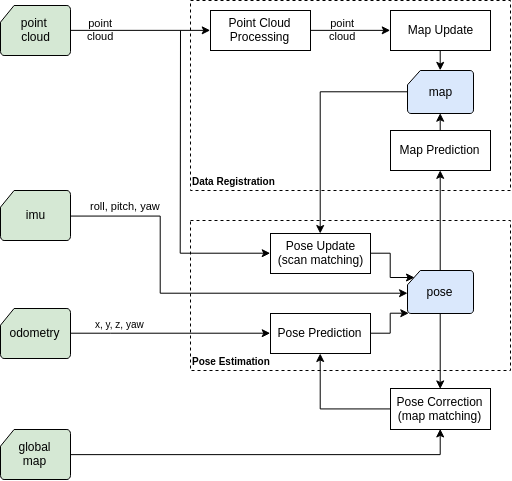
\includegraphics[scale=0.4,draft]{high_level_design_diagram}
    % \includegraphics[scale=0.4]{scenario_4_terrain}
    \caption[Name]{
        Description
    }
    \label{fig:terrain_4}
\end{figure}

\begin{figure}
    \centering
    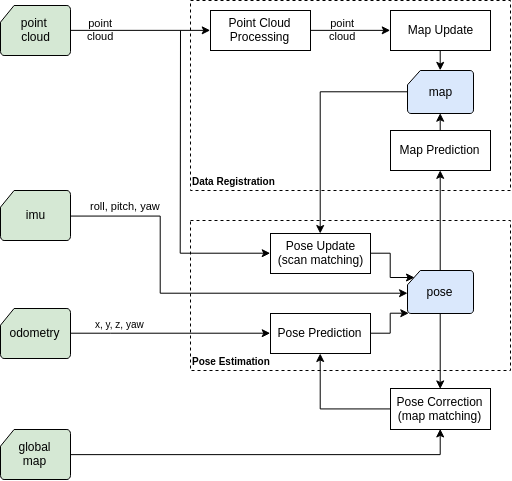
\includegraphics[scale=0.4,draft]{high_level_design_diagram}
    % \includegraphics[scale=0.4]{scenario_4_bird}
    \caption[Name]{
        Description
    }
    \label{fig:bird_3}
\end{figure}

\begin{figure}
    \centering
    % This file was created by matplotlib2tikz v0.6.15.
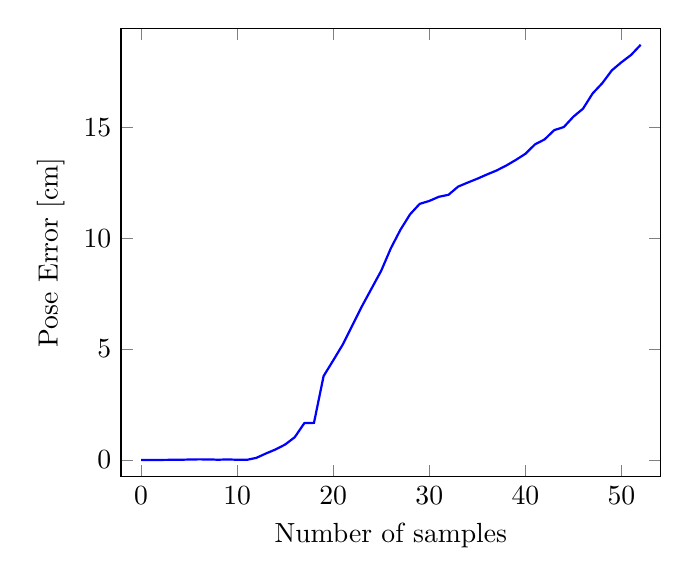
\begin{tikzpicture}

\begin{axis}[
xlabel={Number of samples},
ylabel={Pose Error [cm]},
xmin=-2.08, xmax=54.08,
ymin=-0.748415252462355, ymax=19.4588330238832,
axis on top,
tick pos=both
]
\addplot [thick, blue, forget plot]
table {%
0 1.35036525754666e-06
1 0.000125138484529261
2 0.00102913069024886
3 0.00479680696188859
4 0.00916186830903526
5 0.0174038646274569
6 0.0262520837326282
7 0.0221047623524557
8 0.0111512199617931
9 0.0201210813050887
10 0.0103041075482047
11 0.00407634710390544
12 0.0926150953094736
13 0.290839276112037
14 0.472058763443635
15 0.694965291952438
16 1.02500944562528
17 1.66024002284578
18 1.6709268730271
19 3.77884873435007
20 4.48456421300077
21 5.20350845261926
22 6.06989521034351
23 6.93276612800943
24 7.7323716638851
25 8.52934043849111
26 9.54013041030872
27 10.3761549548947
28 11.070579373762
29 11.5411081034943
30 11.6740911712709
31 11.8615182982339
32 11.9506618950995
33 12.319284997278
34 12.5018994038963
35 12.6755111193714
36 12.8659334573785
37 13.0459756265849
38 13.2666821205177
39 13.5203293101627
40 13.796881010613
41 14.2231742569443
42 14.4465486146409
43 14.8645806490604
44 15.0041899388582
45 15.4721867591002
46 15.8327233804673
47 16.518800150712
48 16.9798252351286
49 17.5599615612027
50 17.9252447964595
51 18.2535561358361
52 18.7104164210556
};
\end{axis}

\end{tikzpicture}

    % \input{Plots/pose_correction_error_2.tex}
    \caption[Name]{
        Description
    }
    \label{fig:pose_correction_error_2}
\end{figure}

The lack of features in the terrain is also visible in global
elevation map (Figure \ref{fig:global_elevation_map_2}) and its gradient
(Figure \ref{fig:global_gradient_map_2}).
% TODO: add bird's eye view with: ground truth/no correction/correction
% TODO: add orthographic projection with global elevation map and its gradient

\begin{figure}
    \centering
    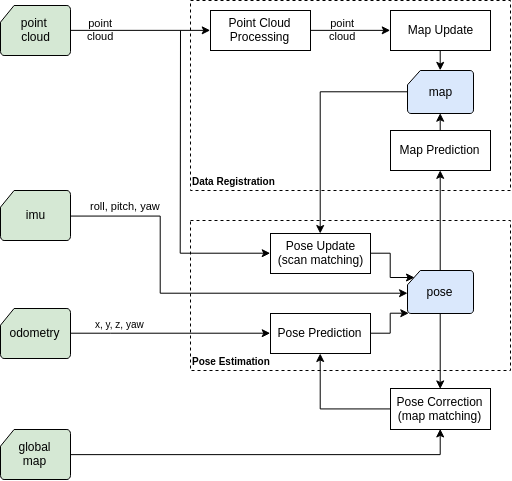
\includegraphics[scale=0.4,draft]{high_level_design_diagram}
    % \includegraphics[scale=0.4]{global_elevation_map_2}
    \caption[Name]{
        Description
    }
    \label{fig:global_elevation_map_2}
\end{figure}

\begin{figure}
    \centering
    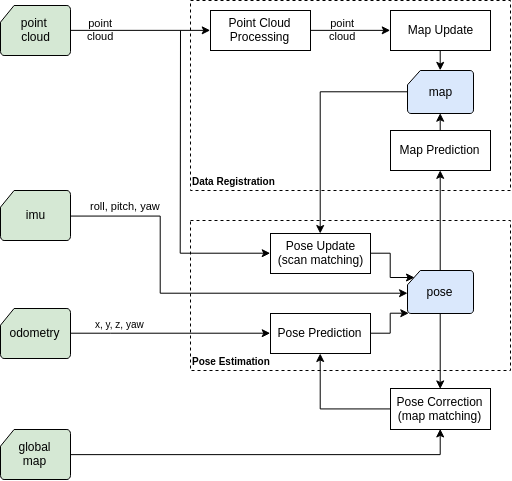
\includegraphics[scale=0.4,draft]{high_level_design_diagram}
    % \includegraphics[scale=0.4]{global_gradient_map_2}
    \caption[Name]{
        Description
    }
    \label{fig:global_gradient_map_2}
\end{figure}

\subsection{Map Resolution Viability}

In this experiment, we validate and measure the performance of our map
matching technique for absolute localization by performing the same
scenarios with different combinations of resolutions for the local and
global maps.
This is done with the aim to draw conclusions regarding the viability
of our approach w.r.t. the available global map data as well as
the processing capabilities of a robot.

Figure \ref{fig:map_resolutions} presents the local and global elevation
maps with distinct resolution values.
Upon matching these maps, we observe the score of each match for every
combination of resolutions (Table \ref{table:map_resolutions}).
% TODO: quickly discuss result

\begin{figure}
    \centering
    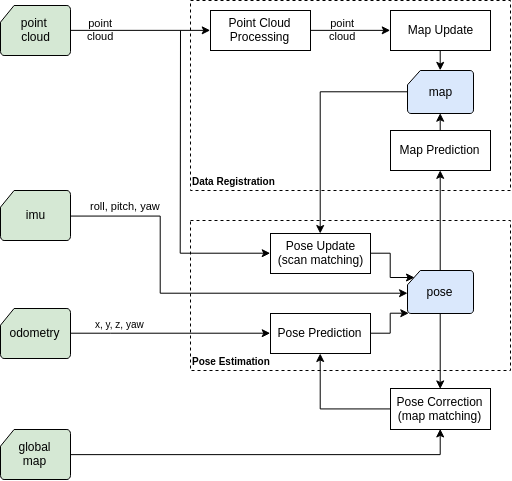
\includegraphics[scale=0.4,draft]{high_level_design_diagram}
    % \includegraphics[scale=0.4]{map_resolutions}
    \caption[Name]{
        Description
    }
    \label{fig:map_resolutions}
\end{figure}

% TODO: move this paragraph to Conclusion
Although the size and resolution of the local map are parameters that we
determine, they are highly limited by the on board processing power of the
robot, since the higher the resolution the more computations must be performed.
On the other hand, the resolution of the global map is a parameter that is
determined by the equipped camera sensors of the orbiters and the
reconstruction techniques applied to the imagery received from those.
As the technology of the space industry advances, we can expect to observe
in the next few years an increase in the aforementioned resolution parameters
and, consequently, an increase in efficiency of the map matching techniques.
As an example, the HiRISE on board camera of the
\textit{Mars Reconnaissance Orbiter} can currently achieve a resolution of
$\SI{30}{\cm \per pixel}$ with the possibility to acquire stereo image pairs
with a precision better than $\SI{25}{\cm \per pixel}$ over locations of
high priority, i.e. potential landing site of future missions to Mars.
% TODO(ref): HiRISE fact

